\begin{figure*}
 \centering % avoid the use of \begin{center}...\end{center} and use \centering instead (more compact)
 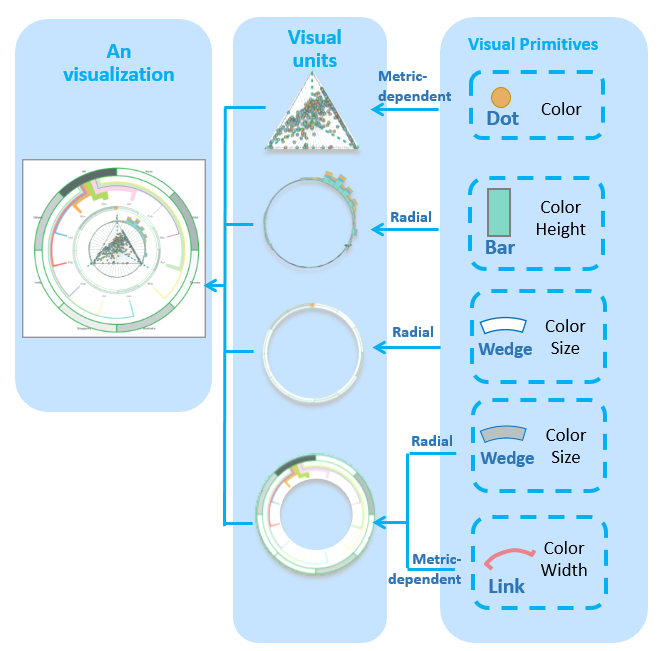
\includegraphics[width=\linewidth]{hierarchic}
 \caption{An example of the hierarchical structure of a visualization, Opinion Seer\cite{wu_opinionseer:_2010}}
 \label{fig:hierarchic}
\end{figure*}

\begin{figure}[tb]
 \centering % avoid the use of \begin{center}...\end{center} and use \centering instead (more compact)
 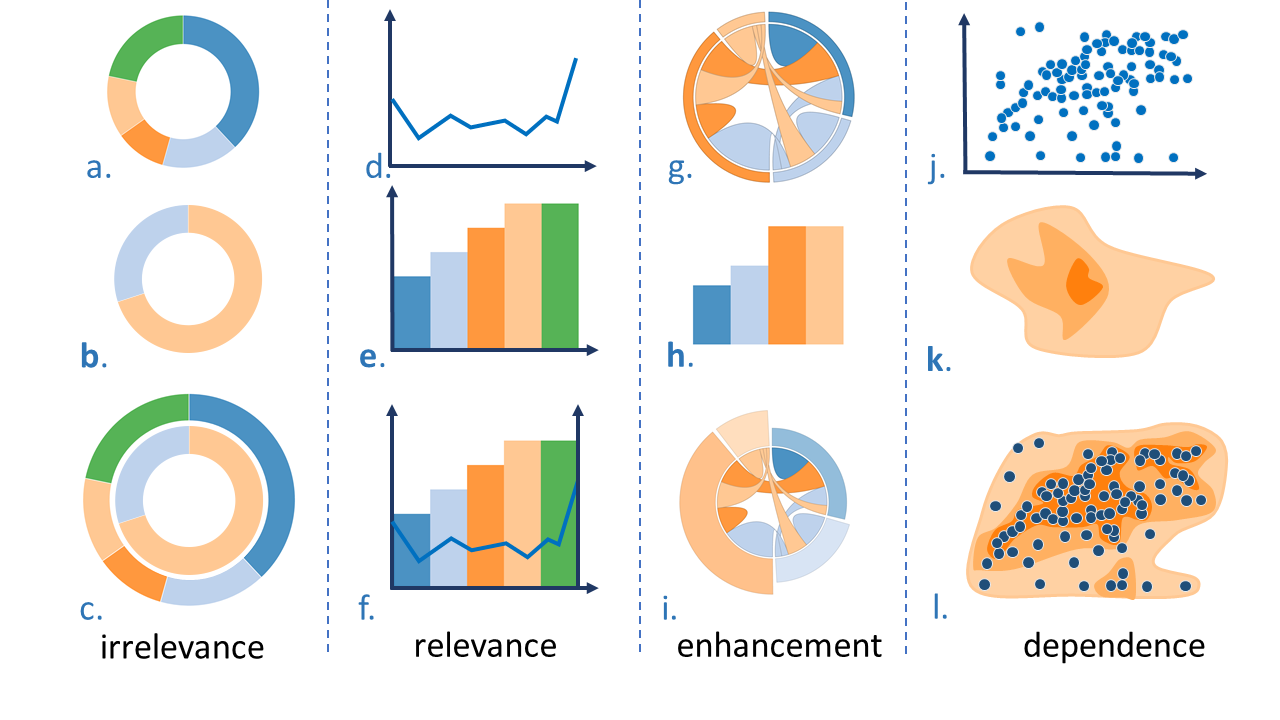
\includegraphics[width=\columnwidth]{unit_relationship}
 \caption{Illustration of the two kinds of relationship between visual units}
 \label{fig:unit_relationship}
\end{figure}

\section{Introducing A Data Visualization} \label{analysis}

To help people better understand a data visualization design, we propose a model that introduces a data visualization through constructing, which has been proven as an effective teaching method\cite{huron_constructive_2014, chapman_constructive_1988}. To build a constructive model for presenting visual designs, there are three questions we need to answer: ``\textit{what are the basic components that compose a data visualization? }'' ,``\textit{what is the relationship between these components? }'', ``\textit{How should we deal with these relationships in our narrative?}''. At the same time, considering a large number of graphical elements employed in a data visualization design, we should eliminate the visual distraction to keep audience's focus on the target.

We propose this model based on our observation of the 375 text visualizations collected and classified in the survey made by Kucher~\cite{kucher2015text}, as well as the lessons from previous work. 

\subsection{Compositions of a Visualization}\label{compositions}
Several work has taken efforts to identify the atomic building blocks of a visualization~\cite{mendez_ivolver:_2016, bertin1983semiology}. 
This model is the extension of previous work by 1) including the relationship bet. 
In our model, a visualization is decomposed into a hierarchical structure of three levels, including
% three levels of structure: 
visual primitives, visual units, and an advanced visualization design. 
% For example, we apply this hierarchical structure theory to 
Taking OpinionSeer~\cite{wu_opinionseer:_2010} as an example, we apply the hierarchical model and decompose it into five visual units, as shown in Figure~\ref{fig:hierarchic}. 

\textbf{A visual primitive} is one graphical element whose visual channels, such as color, width, height, are mapped to data attributes with certain visual grammars. Visual channels are visual properties that control the appearance of a graphical element, and a visual grammar describes how a visual channel indicates a data attribute. For instance, a point is a visual primitive, size is a visual channel, and``size indicates the importance score'' is a visual grammar. 

\textbf{A visual unit} is the assembly of one kind of visual primitives based on a certain construction rule, as Table~\ref{tab:unit} show. Considering the fact that new designs are appearing continually, the purpose of this table is not to cover all visual units but to demonstrate how a visual unit can fit in a table cell.
%For the taxonomy of constructing rule, we refer the ``alignment method'' in \cite{kucher2015text} but make it more specific. 
Visual primitives of one kind can constitute different visual units by following different construction rules. For example, dots can constitute scatter plot, spiral dot chart, or circle packing chart by following radial, orthogonal, or metric-based construction rules, respectively. 
A visual unit is the smallest functional unit of a visualization. 
%\original{Note that we only consider statical visualization.}\siwei{mention it in limitations} People might employ several visual primitives in an animated visualization unit.\siwei{in the first sentence, you said a visual unit is the assemble of ONE kind of... revise it.} For example, Huron et al.~\cite{huron_visual_2013} employed two visual primitives to mimic the physical process of sedimentation for visualizing data streams. 

\textbf{A visualization} can be treated as the combination of visual units. A simple visualization contains only one visual unit while an advanced one is usually the combination of multiple visual units. 
%It doesn't simply put all visual units together but constructs them based on their relationships, as described in Section 3.2.1.
% with certain connections \siwei{what is certain connections? can you give an example?} with each other, which is detailedly discussed in section 3.1.2.\siwei{where is section 3.1.2?}



%\begin{figure}
%\begin{minipage}{\columnwidth}
% \centering % avoid the use of \begin{center}...\end{center} and use \centering instead (more compact)
% 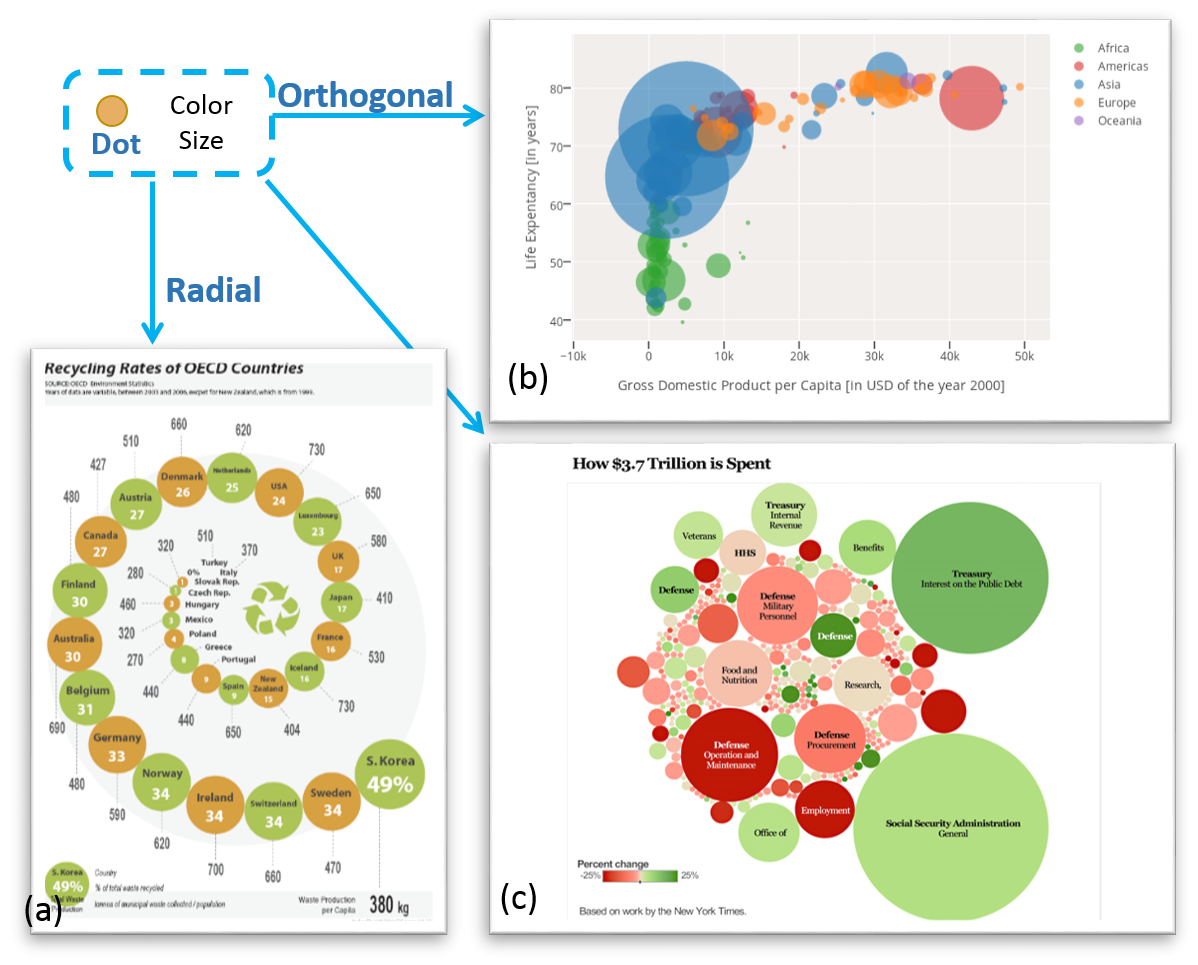
\includegraphics[width=\columnwidth]{assemble}
%\caption[assemble]
%{
%A dot, whose color and size are encoded, can assemble 
%(a) a dot spiral chart
%\protect\footnotemark{}
%    , (b)a dot packing chart
%  \footnotemark{}
%  , and (c)a bubble chart
%  \footnotemark{}
%   by following different construction rules.
%}
%\end{minipage}
%\label{fig:hierarchic}
%\end{figure}
%\footnotetext{https://www.pinterest.com/pin/16536723602037537/}
%\footnotetext{https://plot.ly/~etpinard/84.embed}
%\footnotetext{https://bl.ocks.org/mbostock/4063269}

%\begin{table*}[tb]
%  \caption{A taxonomy of visual units.\notsure{How to avoid the name ambiguities}}
%  \label{unit}
%  \small
%  \centering
%  \begin{tabular}{|p{1.2cm}|p{1.2cm}|p{1.2cm}|p{1.2cm}|p{1.2cm}|p{1.2cm}|p{1.2cm}|p{1.2cm}|p{1.2cm}|}
%  \toprule
%   \textbf{} &\multicolumn{2}{|c|}{Polar Coordinates} &\multicolumn{3}{|c|}{Orthogonal Coordinates}&\multicolumn{3}{|c|}{Metric Dependent}   \\ 
%  \midrule
%  
% \textbf{} &\textbf{Radial} &\textbf{Spiral} &\textbf{Orthogonal} & \textbf{Parallel Align}&\textbf{Map}&\textbf{Cluster}&\textbf{Force-direct}&\textbf{Others}   \\ 
%  \midrule
%  \textbf{Dot} &    &Spiral Dot Chart&Scatter Plot, Bubble Chart & Dot Plot & Bubble Map &  Circle packing    &TopicPanorama\cite{7042494}  &    \\
%  \midrule
%  \textbf{Line}&  Radar Chart   &  Spiral Plot    &Node-link Diagram, Line Chart & Parallel Coordinates, Arc Diagram &    &   &     & \\ 
%  \midrule
%   \textbf{Flow}&  Chord Diagram   &    & &Parallel Sets, Sankey Diagram & 
%   Flow Map  &   &   &\\
%  \midrule
%  \textbf{Area}&    &Area Spiral Chart &Stream Graph &  & & &   &\\ 
%  \midrule
%  \textbf{Bar}&      Radial Bar Chart & Spiral Bar Chart  & Candlestick Chart & Bar Chart  &    &    &    &\\
%  \midrule
%  \textbf{Cell}& Sunburst Diagram  &    & Matrix, Tree Map &     & & &   &\\
%  \midrule
%  \textbf{Wedge}& Pie Chart, Donut Chart &  &   &   &  &    &   &\\
%  \midrule
%  \textbf{Text}&    &Parallel Tag Cloud \cite{collins2009parallel} &    &  Sentence Tree  &     &Word Cloud  &   &    \\
%  %\midrule
% % \textbf{Image}& & &Heatmap Matrix &Heatmap &\\
%  \bottomrule
%  
%  \end{tabular}
%  \vspace{1mm}
%\end{table*}

\begin{table}[tb]
  \caption{A taxonomy of visual units.}
  \label{tab:unit}
  \small
  \centering
  \begin{tabular}{p{0.8cm}|p{2.0cm}|p{2.0cm}|p{2.0cm}}
  \toprule
%  \textbf{} &\multicolumn{2}{|c|}{\textbf{Absolute Position}} &\textbf{Relative Position}   \\ 
%  \midrule
 \textbf{} &\textbf{Radial} &\textbf{Orthogonal, Align, Map} &\textbf{Metric-based}   \\ 
  \midrule
  \textbf{Dot} &Spiral&Dot Chart, Scatter Plot, Bubble Chart, Bubble Map &Circle packing, TopicPanorama\cite{7042494}\\
  \midrule
  \textbf{Line}&  Radar Chart, Spiral Plot    &Line Chart, Parallel Coordinates, Arc Diagram &  Force-directed Node-link graph   \\ 
  \midrule
   \textbf{Flow}&  Chord Diagram   &Parallel Sets, Sankey Diagram, 
   Flow Map  & \\
  \midrule
  \textbf{Area}&  Area Spiral Chart &Stream Graph & Contour Map \\ 
  \midrule
  \textbf{Bar}&      Radial Bar Chart,Spiral Bar Chart  & Candlestick Chart, Bar Chart  &   \\
  \midrule
  \textbf{Cell}& Sunburst Diagram  &Matrix, Tree Map &  \\
  \midrule
  \textbf{Wedge}& Pie Chart, Donut Chart &  &  \\
  \midrule
  \textbf{Text}&  People Spiral in\cite{dork_visual_2010}  &  Sentence Tree  & Word Cloud \\
  %\midrule
 % \textbf{Image}& & &Heatmap Matrix &Heatmap &\\
  \bottomrule
  
  \end{tabular}
  \vspace{1mm}
\end{table}

\subsection{Relationships Between Compositions}
\label{relationship}
We first describe the relationship between conceptual compositions, then offer suggestions for narrative sequence based on these relationships. Notice that we skip the relationship between visual primitives since there is only one kind of visual primitives in a visual unit. 



\subsubsection{Relationships Between Visual Units}
A visualization can be specified as the combination of several visual units. 
% Through observing the approaches people apply to design new visualizations,
We go through all the text visualizations collected in Kucher and Kerren's survey~\cite{kucher2015text}, and identify two types of relationships between visual units: unidirectional relationship and bidirectional relationship. Since visual units are the combination of construction rules and visual primitives, we can describe the relationship between two visual units through describing the relationship between their visual units and constructing rules.  

\textbf{Bidirectional relationship} refers to that the dependency of two visual units is mutual. They share the same construction rule and their visual primitives indicate separate data attributes in a dataset.
For example, in Figure~\ref{fig:relationship}(a) \siwei{citation error} a line chart and  a bar chart are put together with the same construction rule. 

\textbf{Unidirectional relationship} refers to that one visual unit ``A'' depends on another visual unit ``B''.  This dependency is established either by ``replacing'' or ``adding''. A dependency established by ``replacing'' refers to that ``A'' replaces the original graphical elements in ``B'' to build a new visual design. For example, in Figure~\ref{fig:unit_relationship}(b), a bar chart replaces the node segments in a chord diagram. This kind of dependency widely exists in the advanced visualization design, such as the heat map mapped upon the streams in a theme river~\cite{wu_opinionflow:_2014}  and usage of glyphs to replace the nodes in a multidimensional scaling (MDS) plot~\cite{chen_peakvizor:_2016}. A dependency established by ``adding'' means that ``A'' is added to reveal a more detailed description of ``B''. Such description can be the more detailed information from dataset, or information obtained from the previous visualization (Figure~\ref{fig:unit_relationship}(c)). For example, in Figure~\ref{fig:unit_relationship}(c), a contour map is mapped upon a MDS map to illustrate the area with high distribution density, \original{which information is obtained from the MSD map rather than a dataset.}\siwei{this is problematic} While in Figure~\ref{fig:unit_relationship}(d), a donut chart is added to another donut chart, to reveal more hierarchies, \original{which is directly obtained from the dataset. }\siwei{why do you need to emphasize where the information come from?}


A proper narrative sequence of visual units should take these two types of relationships into consideration. For a unidirectional relationship, the dependent should be explained after the visual unit it depends on. For a bidirectional relationship, these two visual units should be explained together but the sequence can be arbitrary. 
We display relationships between units through a tree diagram where every visual unit is represented by a tree node. Sibling nodes stand for visual units with a bidirectional relationship while a child node and a parent node stand for two visual units that have a unidirectional relationship. A proper narrative sequence can be obtained by running a deep first search on this tree diagram. 



\subsubsection{Relationships Between Visual Channels}
For a visual primitive, different channels are encoded with different data attribute. Thus, they are usually separated and have no logic dependency upon others. It's hard to determine a narrative sequence from their inner logical dependency. 

Therefore, we define two metrics to order the explaining of visual channels: \textbf{the complexity of their encoded information} and \textbf{saliency of their visual appearance}.

First, the order of decreasing visual saliency can facilitate graphical perception~\cite{cleveland_graphical_1984}. Even though different channels have intrinsically different perceptual salience and channel with high salience will suppress the expression of other, such salience strength can be influenced in a task-dependent manner ~\cite{nothdurft_salience_2000}. By introducing the channel with high saliency first, we remove it from the task list in our mind~\cite{itti2001computational}, decrease its saliency and give other channels more chance to attract the limited human attention. 

Second, the order of increasing complexity leads to an effective learning process. “Easy to difficult” practice has been long used and confirmed to be effective for learning new tasks~\cite{bliss_effects_1992}.
 
The visual saliency of different channels is relatively constant and  well defined ~\cite{munzner_visualization_2014,cleveland_graphical_1984}, while their information complexity varies in different designs. And an effective narrative sequence is a trade-off between these two metrics. 

%\subsubsection{Non-linear Sequence}
%So far, all the narrative explanation we discussed is linear. However, reading a lengthy, extremely detailed instruction maybe tedious. A good narrative explanation should include non-linear design, allowing users to skip uninterested parts, go back to previous information and freely switch between different parts. Also, users should be allowed the flexibility to choose explanations at different levels of details. 

\subsection{Attention Orientation}
To keep audiences focusing on the target object, it is necessary to identify visual distractions so that measurements can be taken to avoid them. 
We identify two kinds of visual distractions: the one from context and the one from sibling channels, which refer to the visual channels belonging to the same visual primitives. 

\subsubsection{Visual Distraction from the Context}
This kind of distraction has been widely discussed in the field of object detection and human visual attention ~\cite{nothdurft_salience_2000, standage_modelling_2005}. Its intensity is mainly  determined by spatial distance and appearance similarity ~\cite{wolfe_guided_1994}. 
Focus + Context, which might be the most popular techniques for this problem, make uneven use of graphic resources to discriminate focus from their context. At the same time, adding dynamic changes to focus elements has also been demonstrated as effective under various conditions\cite{waldner_attractive_2014}. We support easy implementation of these techniques in our system. 

\subsubsection{Visual Distraction from Sibling Channels}
A visual primitive usually has more than one visual channels. Thus, when recognizing one primitive, the channels with high visual saliency can significantly influence the expression of other channels. For example, color can be a strong noise when the focus is supposed to be the shape. By exaggerating or suppressing certain visual channels, we try to reduce such distractions.


